\chapter{Implementation}\label{ch:implementation}
\epigraph{\textit{ \normalsize“The portion of evolution in which animals developed eyes was a big development. Now computers have eyes.”}}{\normalsize\textit{Jeff Dean,\\ Lead of Google Brain}}

% Implementation details

The first step is to implement the state-of-the-art in image regeneration to guage the improvements. We use DCGAN to start of with. The results of the training and testing will be recorded to compare it with the results of our CapsNet-based approach later. We will be using CapsNet as the underlying technology to implement our GAN (CapsGAN). The goal is to replace the CNN inside DCGAN with CapsNet and compare the results. The GAN internally consists of two components - a generator and a discriminator - which we build out of CapsNet. The discriminator is initially trained separately to distinguish between real and fake data, and later they work together to improve upon their performance by acting as adversaries.
\par\bigskip

\begin{figure}[H]
\centering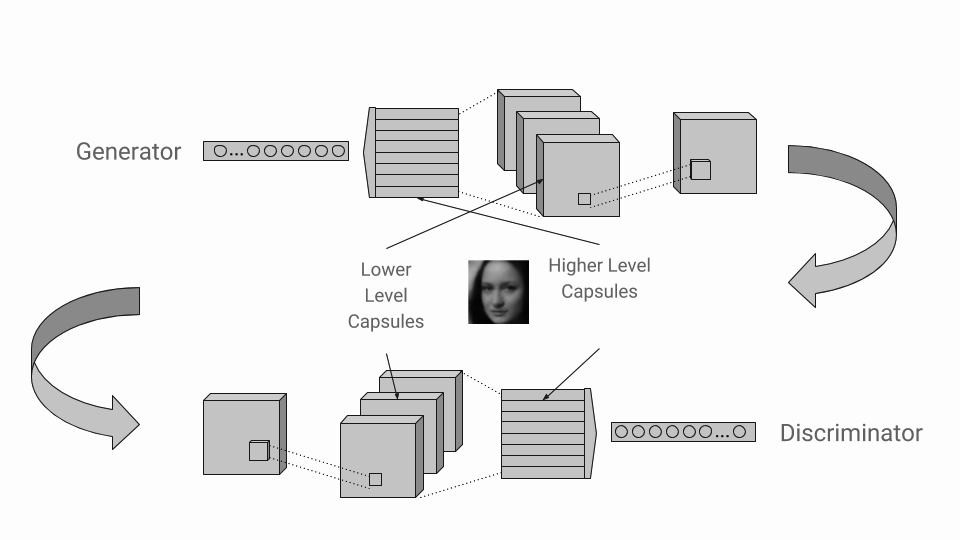
\includegraphics[width=1\textwidth]{images/methodology.png}
\caption{CapsDCGAN Architecture}
\label{fig:capsgan}
\end{figure}

During the course of our research we were forced to conclude that building a CapsNet based generator was not feasible. A fundamental aspect of CapsNet is dynamic routing which is not possible to replicate in the generator, that is, dynamic routing cannot be inverted. Hence we implemented just the discriminator in CapsNet. 
\par\bigskip

We concentrated on four networks: DCGAN, WGAN, ACGAN and InfoGAN. Our training laboratory was Colaboratory - the cloud machine learning research platform. We trained each network individually for 20,000 epochs each. For our preliminary training we used the MNIST dataset \cite{mnist}. The MNIST dataset is a large dataset of handwritten digits commonly used for image processing training tasks. Each of the networks had it's discriminator augmented with the CapsNet code. The networks with the CapsNet discriminator were then individually trained on the same dataset, for 20,000 epochs each. Overall, it took us a few days to train all the networks and gather all the data.
\par\bigskip

\section{Network Architectures} % (fold)
\label{sec:network_architectures}
The following are the network architectures of the generator and the discriminator.

\subsection{Generator} % (fold)
\label{sub:generator}
\begin{lstlisting}[basicstyle=\scriptsize,language=Python]
_________________________________________________________________
Layer (type)                 Output Shape              Param #   
=================================================================
dense_5 (Dense)              (None, 8192)              827392    
_________________________________________________________________
reshape_1 (Reshape)          (None, 8, 8, 128)         0         
_________________________________________________________________
batch_normalization_3 (Batch (None, 8, 8, 128)         512       
_________________________________________________________________
up_sampling2d_1 (UpSampling2 (None, 16, 16, 128)       0         
_________________________________________________________________
conv2d_1 (Conv2D)            (None, 16, 16, 128)       147584    
_________________________________________________________________
activation_1 (Activation)    (None, 16, 16, 128)       0         
_________________________________________________________________
batch_normalization_4 (Batch (None, 16, 16, 128)       512       
_________________________________________________________________
up_sampling2d_2 (UpSampling2 (None, 32, 32, 128)       0         
_________________________________________________________________
conv2d_2 (Conv2D)            (None, 32, 32, 64)        73792     
_________________________________________________________________
activation_2 (Activation)    (None, 32, 32, 64)        0         
_________________________________________________________________
batch_normalization_5 (Batch (None, 32, 32, 64)        256       
_________________________________________________________________
up_sampling2d_3 (UpSampling2 (None, 64, 64, 64)        0         
_________________________________________________________________
conv2d_3 (Conv2D)            (None, 64, 64, 32)        18464     
_________________________________________________________________
activation_3 (Activation)    (None, 64, 64, 32)        0         
_________________________________________________________________
batch_normalization_6 (Batch (None, 64, 64, 32)        128       
_________________________________________________________________
conv2d_4 (Conv2D)            (None, 64, 64, 3)         867       
_________________________________________________________________
activation_4 (Activation)    (None, 64, 64, 3)         0         
=================================================================
Total params: 1,069,507
Trainable params: 1,068,803
Non-trainable params: 704
_________________________________________________________________
\end{lstlisting}
% subsection generator (end)

\subsection{Discriminator} % (fold)
\label{sub:discriminator}
\begin{lstlisting}[basicstyle=\scriptsize,language=Python]
____________________________________________________________________________________________
Layer (type)                    Output Shape         Param #     Connected to               
============================================================================================
input_1 (InputLayer)            (None, 64, 64, 3)    0                                      
____________________________________________________________________________________________
conv1 (Conv2D)                  (None, 56, 56, 256)  62464       input_1[0][0]              
____________________________________________________________________________________________
leaky_re_lu_1 (LeakyReLU)       (None, 56, 56, 256)  0           conv1[0][0]                
____________________________________________________________________________________________
batch_normalization_1 (BatchNor (None, 56, 56, 256)  1024        leaky_re_lu_1[0][0]        
____________________________________________________________________________________________
primarycap_conv2 (Conv2D)       (None, 24, 24, 256)  5308672     batch_normalization_1[0][0]
____________________________________________________________________________________________
primarycap_reshape (Reshape)    (None, 18432, 8)     0           primarycap_conv2[0][0]     
____________________________________________________________________________________________
primarycap_squash (Lambda)      (None, 18432, 8)     0           primarycap_reshape[0][0]   
____________________________________________________________________________________________
batch_normalization_2 (BatchNor (None, 18432, 8)     32          primarycap_squash[0][0]    
____________________________________________________________________________________________
flatten_1 (Flatten)             (None, 147456)       0           batch_normalization_2[0][0]
____________________________________________________________________________________________
uhat_digitcaps (Dense)          (None, 160)          23593120    flatten_1[0][0]            
____________________________________________________________________________________________
softmax_digitcaps1 (Activation) (None, 160)          0           uhat_digitcaps[0][0]       
____________________________________________________________________________________________
dense_1 (Dense)                 (None, 160)          25760       softmax_digitcaps1[0][0]   
____________________________________________________________________________________________
multiply_1 (Multiply)           (None, 160)          0           uhat_digitcaps[0][0]       
                                                                 dense_1[0][0]              
____________________________________________________________________________________________
leaky_re_lu_2 (LeakyReLU)       (None, 160)          0           multiply_1[0][0]           
____________________________________________________________________________________________
softmax_digitcaps2 (Activation) (None, 160)          0           leaky_re_lu_2[0][0]        
____________________________________________________________________________________________
dense_2 (Dense)                 (None, 160)          25760       softmax_digitcaps2[0][0]   
____________________________________________________________________________________________
multiply_2 (Multiply)           (None, 160)          0           uhat_digitcaps[0][0]       
                                                                 dense_2[0][0]              
____________________________________________________________________________________________
leaky_re_lu_3 (LeakyReLU)       (None, 160)          0           multiply_2[0][0]           
____________________________________________________________________________________________
softmax_digitcaps3 (Activation) (None, 160)          0           leaky_re_lu_3[0][0]        
____________________________________________________________________________________________
dense_3 (Dense)                 (None, 160)          25760       softmax_digitcaps3[0][0]   
____________________________________________________________________________________________
multiply_3 (Multiply)           (None, 160)          0           uhat_digitcaps[0][0]       
                                                                 dense_3[0][0]              
____________________________________________________________________________________________
leaky_re_lu_4 (LeakyReLU)       (None, 160)          0           multiply_3[0][0]           
____________________________________________________________________________________________
dense_4 (Dense)                 (None, 1)            161         leaky_re_lu_4[0][0]        
============================================================================================
Total params: 29,042,753
Trainable params: 29,042,225
Non-trainable params: 528
____________________________________________________________________________________________
\end{lstlisting}
% subsection discriminator (end)

% section network_architectures (end)

\section{Demonstration} % (fold)
\label{sec:imp_demonstration}
The training of the models took place on Colaboratory, over Keras. Keras provided for a fast implementation of the code and high level abstraction. The output model was in the format of H5. This could not be directly used as part of semantic inpainting as semantic inpainting requires changing low level architectural details which Keras does not allow. Hence we converted the H5 model to TensorFlow protocol buffer, which is TensorFlow's model saving format, the code for which can be found in \ref{sub:converting_models}.
\par\bigskip

For the semantic inpainting, we take as input an image. The image is loaded onto a canvas with an ability to mask a part of the image. Once the mask is set, our processing starts. The following process is based on Raymond A. Yeh \textit{et al.} \cite{inpainting}
\par\bigskip

The masked image is a Hadamard product of the mask component, M, and the original input image, y. 
\begin{equation} \label{eqn:masked_image}
Masked Image = \bm{M} \odot\  \bm{y}
\end{equation}
\par\bigskip

Suppose we've found an image from the generator $G(\hat z)$ for some $\hat z$ that gives a reasonable reconstruction of the missing portions. The completed pixels $(1 - M) \odot G(\hat z)$ can be added to the original pixels to create the reconstructed image:
\begin{equation} \label{eqn:reconstructed_image}
\bm{x} \textsubscript{reconstructed} = \bm{M} \odot\  \bm{y} + (1 - \bm{M}) \odot \bm{G} (\hat z)
\end{equation}
\par\bigskip

Now all that is needed is to find a $G(\hat z)$ that does a good enough job of completing the image. We will consider a loss function, a smaller value of which means that z is more suitable for completion. The total loss function will be a sum of two loss functions: Contextual and Perceptual.

\subsection{Contextual Loss} % (fold)
\label{sub:contextual_loss}
To keep the same context as the input image, make sure the known pixel locations in the input image y are similar to the pixels in $G(z)$. We need to penalize $G(z)$ for not creating a similar image for the pixels that we know about. Formally, we do this by element-wise subtracting the pixels in $y$ from $G(z)$ and looking at how much they differ:
\begin{equation} \label{eqn:contextual_loss}
\bm{L}\textsubscript{contextual}(\bm{z}) = || \bm{M} \odot\  \bm{G(m)} + (1 - \bm{M}) \odot \bm{G} (\hat z) || \textsubscript{1}
\end{equation}
where $||x|| \textsubscript{1}=\sum \textsubscript{i} |x \textsubscript{i}|$ is the $l \textsubscript{1}$ norm of some vector $x$.

% subsection contextual_loss (end)

\subsection{Perceptual Loss} % (fold)
\label{sub:perceptual_loss}
To recover an image that looks real, let’s make sure the discriminator is properly convinced that the image looks real. We’ll do this with the same criterion used in training the network:
\begin{equation} \label{eqn:perceptual_loss}
\bm{L}\textsubscript{perceptual}(\bm{z}) = \bm{log} (1 - \bm{D}(\bm{G}(\bm{z})))
\end{equation}
% subsection perceptual_loss (end)

\subsection{Total Loss} % (fold)
\label{sub:total_loss}
We now find $\hat z$ with a combination of the contextual and perceptual losses:
\begin{equation} \label{eqn:total_loss}
\bm{L}(\bm{z}) = \bm{L}\textsubscript{contextual}(\bm{z}) + \lambda \bm{L}\textsubscript{perceptual}(\bm{z})
\end{equation}
\begin{equation} \label{eqn:minimization}
\hat z = arg \min_z \bm{L} (\bm{z})
\end{equation}

where $\lambda$ is a hyper-parameter that controls how important the contextual loss is relative to the perceptual loss. Then, as before, the reconstructed image fills in the missing values of $\bm{y}$ with $\bm{G}(\bm{z})$:
\begin{equation} \label{eqn:reconstructed_image_final}
\bm{x} \textsubscript{reconstructed} = \bm{M} \odot\  \bm{y} + (1 - \bm{M}) \odot \bm{G} (\hat z)
\end{equation}
% subsection total_loss (end)

\subsection{Projected Gradient Descent} % (fold)
\label{sub:projected_gradient_descent}
	For minimizing the loss function we use projected gradient descent. Its different from gradient descent in the sense, at a basic level, projected gradient descent is just a more general method for solving a more general problem. Gradient descent minimizes a function by moving in the negative gradient direction at each step. There is no constraint on the variable. 
\begin{equation} \label{eqn:gradient_descent}
\text{Problem 1:} \min_x f(x)
$$
$$
x_{k+1} = x_k - t_k \nabla f(x_k)
\end{equation}

On the other hand, projected gradient descent minimizes a function subject to a constraint. At each step we move in the direction of the negative gradient, and then "project" onto the feasible set.

\begin{equation} \label{eqn:projected_gradient_descent}
\text{Problem 2:} \min_x f(x) \text{ subject to } x \in C
$$
$$
y_{k+1} = x_k - t_k \nabla f(x_k)
$$
$$
x_{k+1} = \text{arg} \min_{x \in C} \|y_{k+1}-x\| 
\end{equation}

% subsection projected_gradient_descent (end)

% section demonstration (end)